\chapter{Results}
To test the algorithm's performance I ran it with the following example:

Consider the following Riccati equation with initial condition $y(0) = 1$
\begin{equation*}
    \frac{dy}{dt} = (2 - sin(t)) \cdot y^2 + \frac{2 - sin(t) + cos(t)}{2 - sin(t)} \cdot y - \frac{1}{2 - sin(t)}
\end{equation*}

The following four figures visualize the results of both the classical solver (\textit{y(t)}) and QRS (\textit{z(t)}) over a time period \textit{t} with the classical yt-graph from Differential Equations.

Figure 5.1 depicts the solutions of a classical solver and Figure 5.2 the solutions of QRS for a time step of 0.001. Note that the equation has a singularity, a point in which the solution splits to $\infty$ and $-\infty$, at $t \approx 0.40$ which describes the end of our particular solution. 

\begin{figure}[b]
    \centering
    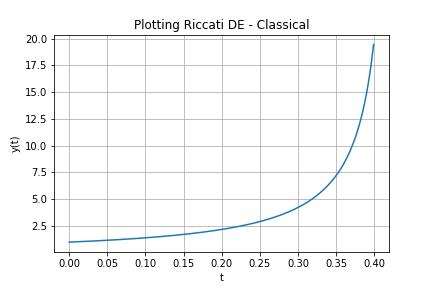
\includegraphics[scale=0.75]{images/Classical_R2.jpg}
    \caption{Classical solver qualitative analysis}
    \label{fig:my_label}
\end{figure}
\begin{figure}[b]
    \centering
    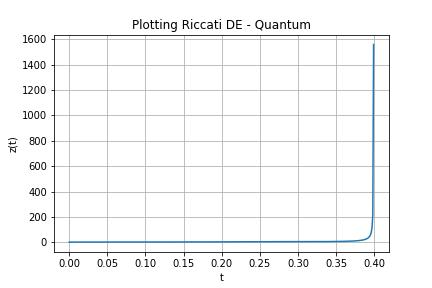
\includegraphics[scale=0.75]{images/Quantum_R2.jpg}
    \caption{Hybrid-Quantum solver qualitative analysis}
    \label{fig:my_label}
\end{figure}

Recall the Uniqueness and Existence theorem states that there is a unique solution for a given initial value problem within a local neighbourhood, defined by $\epsilon > 0$. Zooming into a local neighbourhood at (0.3, 0.375), Figure 5.3 and 5.4 show that QRS provides really good approximations over the specified region with a time step of 0.001.
\begin{figure}[b]
    \centering
    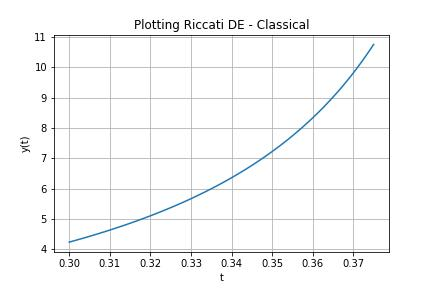
\includegraphics[scale=0.75]{images/Classical_R2_Zoom.jpg}
    \caption{Classical solution in local neighbourhood}
    \label{fig:my_label}
\end{figure}
\begin{figure}[b]
    \centering
    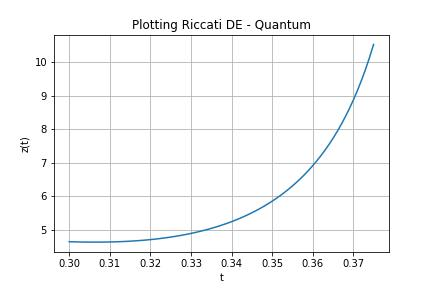
\includegraphics[scale=0.75]{images/Quantum_R2_Zoom.jpg}
    \caption{QRS solution in local neighbourhood}
    \label{fig:my_label}
\end{figure}

I believe the slight variations are mainly due to quantum noise and the singularities inherent to the equations chosen for evaluation. There has been some work on how to address singularities which seem to be common in Riccati equations, Davey \cite{DAVEY1979137} suggests that these could be removed by considering the differential equations for the numerators and the denominators separately of the elements of the Matrix Riccati and its inverse. My thought is that, while attempting to compute numbers growing to $\infty$ the quantum hardware heats up faster; I believe this alteration of the environment may affect the state of the qubits and thus the calculations. Therefore, QRS has a lot of room for improvement by applying error correction techniques and other quantum optimization methods. Further improvements will be discussed in the following section.